\title{Operating Systems–2: CS3523 2019\\
Programming Assignment 2: \\
Implementing TAS, CAS and Bounded Waiting CAS
Mutual Exclusion Algorithms \\
Report}
\author{Sai Harsha Kottapalli\\CS17BTECH11036}
\date{February 17, 2019}

\documentclass[12pt]{article}
\usepackage{graphicx}

\begin{document}
\maketitle

\section{Aim}
The goal of this assignment is to implement TAS, CAS and Bounded Waiting with CAS
mutual exclusion (ME) algorithms studied in the class. Implement these algorithms in C++.

\section{Design of the Program :}
We use three types of algo's as mentioned in the aim, to give access to critical section for threads.
\subsection{Critical Section :}
This part of the code should be accessed by only one thread at a time or as an atomic equivalent.
We can avoid race conditions by making sure that no two processes enter their Critical Sections at the same time.
\subsection{Entry Section :}
This part of the code is accessible for all the threads. The job of this code is to make sure only one thread is given access to the critical section at a particular time.
$\textbf{Note:}$ starvation might occur in case of TAS and CAS algorithm but in case of CAS-bounded algorithm all threads are given a chance to run fairly often when compared to previous algorithms.
\subsection{Exit Section :}
This part of the code is where the thread has successfully executed the critical section of the program, and will reset the lock so that other threads can now enter the critical section(if any) while this thread completed the remainder section parallelly.
\subsection{Worst Time Taken:}
This is defined as the maximum amount of time a thread has to wait after requesting access to the critical section and the access being granted.
\subsection{Average Waiting Time :}
This is defined as the amount of time each access to critical section takes after requesting for the same.

\section{Explanation of program - Common Part}

\subsection{Header files used}
\begin{itemize}
\item iostream\\
Header that defines the standard input/output stream objects
\item thread\\
Used for implementing threads.\\
It defines the class to represent individual threads of execution.\\
A thread of execution is a sequence of instructions that can be executed concurrently with other such sequences in multithreading environments, while sharing a same address space.\\
\item fstream\\
Input/output stream class to operate on files.
\item random\\
This header introduces random number generation facilities.\\
\item atomic\\
Atomic types are types that acts like a wrapper around  a value whose access is guaranteed to not cause data races and can be used to synchronize memory accesses among different threads.
\item cstdio\\
Used for \textbf{sprintf}, that is, for the format in which the time has to be printed to the log file.
\item unistd.h\\
Used for miscellaneous symbolic constants and types, and declares miscellaneous functions - \\
\textbf{localtime} - which is used to get a structure of time, with hours, minutes and seconds.\\
\textbf{time} - For capturing current time which is processed by above command.
\item string\\
For processing strings.
\end{itemize}

\subsection{getInput()}
This is a helper function which helps in keeping the code modular.\\
It reads the value of the following from the input file, specified in ReadMe.txt \\
\begin{itemize}
\item number of threads\\
\item number of times each thread requires to access the critical section\\
\item lambda1 and lambda2\\
Represents the mean of value of two exponential distribution curves which is to be constructed.
\end{itemize}

\subsection{testCS()}
The testCS function is responsible for the simulation of the critical, entry, exit and remainder section.We also use this function to calculate the average waiting time and worst time taken which is later used as the parameters for the comparisions for the three different algorithms mentioned in the aim.

\subsection{currTime()}
Takes input time$\textunderscore$t structure to generate the time in HH:MM:SS syntax and return this as a string.

\subsection{Other important variables used}
\begin{itemize}
\item exponential$\textunderscore$distribution\\
Produces random non-negative floating-point values x, distributed according to probability density function defined for exponential distribution about the constant rate given as a parameter.
\item default$\textunderscore$random$\textunderscore$engine\\
This is a random number engine class that generates pseudo-random numbers.
\item waiting\\
Dynamic array of bool type, based on number of threads given in input file.
\item thread *th\\
th is the pointer for storing the array of n threads.This will be useful for later calling join to properly exit the threads spawned previously.
\end{itemize}

\section{TAS}
\begin{itemize}
\item lock\\
We use atomic$\langle$bool$\rangle$ and initiate this to \textbf{ATOMIC$\textunderscore$FLAG$\textunderscore$INIT}.
\item exchange\\
\textbf{syntax} - exchange( T$\textunderscore$desired, std::memory$\textunderscore$order order = std::memory$\textunderscore$order$\textunderscore$seq$\textunderscore$cst )\\
Atomically replaces the underlying value with desired. The operation is read-modify-write operation. Memory is affected according to the value of order.\\
We use this to implement our TAS algorithm.
\item return value\\
The value of the atomic variable before the call. 
\end{itemize}

\section{CAS and CAS-Bounded}
\begin{itemize}
\item lock\\
We use atomic$\langle$int$\rangle$ and initiate this to \textbf{0}.\\
\textbf{Note:} use lock(0) instead of lock = 0, as there are some issues with using the latter.
\item compare$\textunderscore$exchange$\textunderscore$strong\\
\textbf{syntax} - compare$\textunderscore$exchange$\textunderscore$strong( T\& expected, T$\textunderscore$desired)\\
Atomically compares the object representation of *this with that of expected, and if those are bitwise-equal, replaces the former with desired (performs read-modify-write operation). Otherwise, loads the actual value stored in *this into expected (performs load operation).
\item return value\\
\textbf{true} if the underlying atomic value was successfully changed, \textbf{false} otherwise.
\item \textbf{Note: }expected must always be reset to 0 after every iteration and the above command also change expected when required conditions are met.
\end{itemize}
\pagebreak
\section{Comparision}
\subsection{Graphs}
\begin{figure}[ht!]
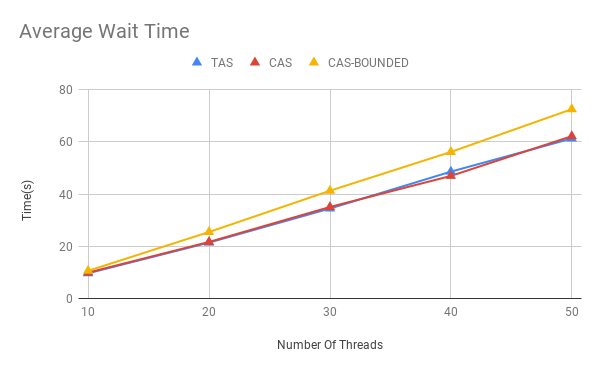
\includegraphics[width=150mm]{Average_Wait_Time.png}
\caption{Comparision between Average time taken for accessing the critical section by the algorithms.}
\end{figure}
\begin{figure}[ht!]
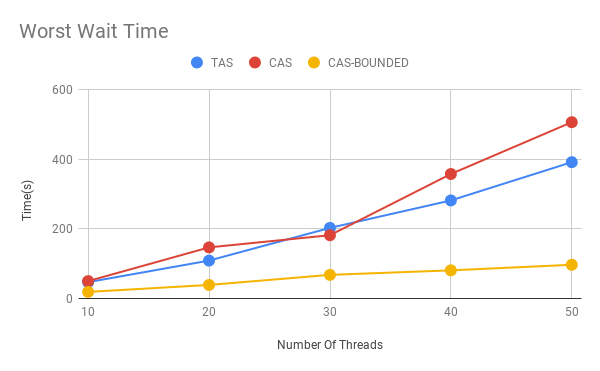
\includegraphics[width=150mm]{Worst_Wait_Time.png}
\caption{Comparision between the worst time taken by the algorithms.}
\end{figure}

\pagebreak
\subsection{Notes}
\begin{itemize}
\item Parameters used for test cases:\\
n = 10, 20, 30, 40 , 50\\
k = 10\\
$\Lambda _1$ = 2 seconds
$\Lambda _2$ = 2 seconds
\item Each of the plotted points is the average of 5 testcases.\\
\item With respect to Average waiting time
Efficiency of algorithms:\\
TAS $\approx$ CAS $>$ CAS-bounded.
\item With respect to Worst time taken
Efficiency of algorithms:\\
CAS-Bounded $>$ TAS $>$ CAS
\end{itemize}

\end{document}